\documentclass[runningheads,a4paper]{llncs}
\usepackage{amssymb}
\usepackage{url}
\usepackage{times}
\usepackage{float}
\usepackage{inconsolata}
\usepackage[T1]{fontenc}
\usepackage{graphicx}
\usepackage{color}
\usepackage{soul}  
\usepackage{nameref}  
\usepackage{amsbsy}  
\usepackage{bezier}  
\usepackage{colortbl}  
\usepackage[leqno,fleqn]{amsmath}  
\usepackage{verbatim}
\usepackage{multicol}
\usepackage{wrapfig}
% deutsche Silbentrennung
\usepackage[ngerman]{babel}
% wegen deutschen Umlauten
\usepackage[utf8]{inputenc}
\usepackage{listings}
\usepackage{epstopdf}

\lstloadlanguages{Ruby}
\lstset{%
  basicstyle=\fontfamily{fi4}\selectfont\color{black},
  commentstyle = \fontfamily{fi4}\selectfont\color{red},
  keywordstyle=\fontfamily{fi4}\selectfont\color{blue},
  stringstyle=\color{green},
  language=Ruby,
  basicstyle=\footnotesize,      % font size
  numbers=left,                  % where to put line numbers
  numberstyle=\footnotesize,     % numbers size
  numbersep=5pt,                 % how far the line numbers are from the code
  backgroundcolor=\color{white}, % background color
  showspaces=false,                          % show spaces (with underscores)
  showstringspaces=false,            % underline spaces within strings
  showtabs=false,                            % show tabs using underscores
  frame=tb,                  % adds a frame around the code
  tabsize=2,                     % default tabsize
  breaklines=true,                  % automatic line breaking
  columns=fullflexible,
  breakautoindent=false,
  framerule=1pt,
  xleftmargin=0pt,
  xrightmargin=0pt,
  breakindent=0pt,
  resetmargins=true,
  stepnumber=1
}


\setcounter{tocdepth}{3}
\newcommand{\keywords}[1]{\par\addvspace\baselineskip
\noindent\keywordname\enspace\ignorespaces#1}

\begin{document}
\mainmatter

\title{Behaviour Driven Development}
\subtitle{Proseminar - Systemanalyse und -design}
\date{Sommersemester 2013}

\author{Steve Dierker}

\institute{
Freie Universit\"at Berlin\\ Institut for Computer Science \\ AG Corporate Semantic Web \\
K\"onigin-Luise-Str. 24/26, 14195 Berlin, Germany\\  dierker.steve@fu-berlin.de \\
\url{http://www.inf.fu-berlin.de/ag-csw}
}

\maketitle

\begin{abstract}
  In dieser Seminararbeit geht es um Behaviour Driven Developent als Sofware 
  Prozess. Insbesondere werden wir uns mit den Gr"unden f"ur die Entwicklung von
  Behaviour Driven Development und den Vor- und Nachteilen zu klassischem Test 
  Driven Development besch"aftigen.\\
  Ein besonderer Fokus wird hier auf ausgew"ahlten Werkzeugen zur Umsetzung von 
  BDD mit der Programmiersprache Ruby gelegt.


\end{abstract}

\keywords{Behaviour Driven Development, Agile Software Process, Ruby, Seminararbeit}

\section{Einleitung}
  BDD ist eine Weiterentwicklung von Test Driven Development und Verkn"upfung 
  mit anderen bestehenden agilen Software Processen wie Domain Driven Design 
  und Object Oriented Analysis.\\
  Programmierer die das erste mal mit TDD in Ber"uhrung kommen brauchen eine 
  lange aufw"arm Phase bis sie effektiv mit diesem Konzept arbeiten k"onnen. 
  Denn bei der Verfolgung dieses Konzeptes stellen sich als erstes zwar simpel 
  erscheinende doch sehr wichtige Fragen.\\
  \begin{itemize}
    \item Was soll getestet werden?
    \item Wo f"angt man mit dem Testen an?
    \item Wieviel sollte ein Test "uberhaupt testen?
    \item Wie sollten Tests benannt sein?
    \item Wie sollte verstanden werden warum ein Test fehlschl"agt?
  \end{itemize}
  Diese Fragen f"uhren zu einer starken Diversit"at zwischen den Umsetzungen
  der Idee von TDD zwischen vielen Programmierer\_innen und erschwert es das Konzept
  schnell und klar an andere Entwickler\_innen weiter zu vermitteln.\\
  Es braucht also eine klar Struktur von 'Best Practises' f"ur TDD um den 
  Umgang mit diesem Prozess zu vereinheitlichen und Anf"angern die M"oglichkeit
  zu geben auch ohne Vorkenntnisse schnell in bestehende Projekt mit diesem 
  Prozess einzusteigen.\\
  Genau diese Probleme, die von Programmierer\_innen die Erfahrung im Umgang mit TDD 
  haben meist umgangen werden indem sie "ahnliche konzeptionelle Methoden wie 
  BDD verfolgen, wurden von Dan North\cite{North:2006} in seinem 
  Artikel erstmals zusammengefasst.\\
  Genau auf diese Konzepte werde ich n"aher eingehen.

\section{Test Driven Development}
  Bevor wir in BDD eintauchen k"onnen m"ussen wir verstehen wie Test Driven 
  Development funktioniert, welche Vortiele es uns bringt und auf welche 
  Probleme wir sto"sen k"onnen.

  \subsection{Red-Green-Refactor}
    Grundlegend ist TDD ein Software Desing Process. Dieser Prozess basiert auf 
    der klaren Mantrik erst Tests f"ur einen nicht existenten Codeabschnitt zu
    schreiben, bevor der Code selbst implementiert wird.\\
    \begin{wrapfigure}{r}{0.5\textwidth}
      \vspace{-30pt}
      \begin{center}
        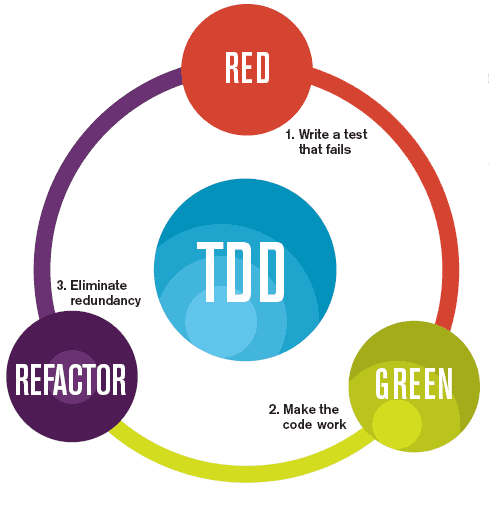
\includegraphics[scale=0.3]{assets/tdd_flow.png}
      \end{center}
      \caption{Red-Green-Refactor\cite{Osorio:2012}}
      \vspace{-15pt}
    \end{wrapfigure}
    Dies wird auch oft als 'Red-Green-Refactor-Zyklus' bezeichnet, da erst der Test
    ausgef"uhrt wird und fehlschl"agt, was bei den meisten Testingframeworks mit 
    Rot markiert wird, nun das Feature implementiert wird und der Test nicht 
    fehlschl"agt -dies wird oft mit Gr"un dargestellt.\\
    Sobald der Test nicht mehr feschl"agt betrachtet man das entstandende Design 
    des Features, reduziert Duplikate und kommentiert seinen Code. Nun kann man 
    ein weiteres mal in den Zyklus eintreten und die n"achsten Features wieder 
    nach dem gleichen System entwicklen.\\
    Ein Zyklus sollte allerdings nicht l"anger als 15 Minuten dauern. Falls doch
    heisst dies entweder das zu implmentierende Feature ist zu gro"s gew"ahlt
    oder der gew"ahlte L"osungsweg nicht optimal ist. Generell 
    sollten sich die Entwickler\_innen immer die Frage stellen ob Debugen 
    schneller als neu implementieren eines Features ist, solange die Tests bei erst
    Implementierung fehlschlagen.

  \subsection{Auswirkungen und Vorteile}
    Sobald die Codebase w"achst wird immer mehr Zeit zum umstrukturieren des 
    bereits entwickelten Quellcodes ben"otigt und es wird sich langsam ein 
    sich konstant weiterentwickelndes Design herauskristallisieren.\\
    Durch diese evolvierende Art des Designs, auch 'Emergent Design'\cite[p.~4]{Chelimsky:2010} genannt, kann sich die Software und somit auch die 
    Entwickler\_innen dynamisch den Anforderungen des Stakeholders anpassen, was 
    besonders in agilen Softwareprozessen n"otig ist. Desweiteren ist es auf 
    Grund der 'Test First' Struktur stets m"oglich ein zumindest begrenzt 
    fertiges Produkt zu pr"asentieren, was sofortige Kommunikation und Feedback
    des Stakeholders erm"oglicht und schnell aufkommende Probleme in der Software
    sichtbar werden l"asst.\\

  \subsection{Bestehende und absehbare Probleme}
    Test Driven Development sollte nicht als Ersatz eines ausf"uhrlichen Testens
    der Software gesehen werden. Eher ist es als Prozess zusehen um qualitativen
    Quellcode an den der Entwicklung angeschlossenen Testzyklus zu "ubergeben.\\
    Doch genau das f"uhrt schnell zur Verwirrungen, da Entwickler\_innen dazu
    neigen TDD als m"oglichkeit zusehen sich diesen extra Testzyklus zu sparen.
    Dies f"uhrt dazu das w"ahrend des Entwickelns neuer Features nicht nur 
    Tests geschrieben werden die das Verhalten des Features nach aussen spezifizieren
    sondern interne technische Details auf Funktion "uberpfr"ufen. Dadurch werden
    die Tests besonders von unerfahrenen TDD-Entwickler\_innen schnell zu 
    ausf"uhrlichem White-Box-Testing genutzt, was zu einer starken Verschr"ankung
    von Test-Suite und eigentlich Quellcode f"uhrt. Durch diese Verschr"ankung
    wird das im Zyklus enthaltene Umstrukturieren des Codes immerweiter 
    erschwert und die Test-Suite verliert an Wartbarkeit, da f"ur das von aussen
    betrachtete Verhalten unwichtige technische Details bei "Anderungen zum 
    fehschlagen der Tests f"uhren k"onnen.\\
    Speziell hierf"ur m"ussen die Entwickler\_innen Disziplin an den Tag legen,
    denn sie sind es die das "aussere Verhalten als Test implementieren und sich
    selbst davon abhalten m"ussen internes Vehalten zu testen.\\
    Ein strukturelles Problem bei TDD ist es, das die Entwickler\_innen selbst
    die Anforderungen der Stakeholder in Tests "ubersetzen m"ussen und es 
    dadurch dazu kommen kann das schon die Tests falsches verhalten pr"ufen
    und somit die Implementierung des Features gar nicht den Anforderungen 
    entsprechen kann. Au"serdem folgt aus der nicht klar gegebenen Nomenklatur
    f"ur Tests, dass sie zwar auf Grund ihrer Funktion das Verhalten der 
    Software dokumentieren, dies allerdings nur auf einer f"ur Entwickler\_innen
    lesbaren Ebene, obwohl nur der Stakeholder verifizieren k"onnnte, das die 
    Tests sein gew"unschtes Verhalten abdecken. Dies kann vielleicht durch 
    Erfahrung der Entwickler\_innen ausgeglichen werden indem sie klare 
    Methodennamen vergeben und durch viele Kommentare auch Menschen die nicht 
    im Programmieren bewandert sind die M"oglichkeit geben die Tests zu 
    verstehene.\\
    Allerdings muss nun jedes neue Teammitglied an diese speziellen Verfahren
    gew"ohnt werden, da sie auf Grund mangelnder Einheitlichkeit stark zwischen
    verschiedenen Teams varieren k"onnen.
    Ausserdem stellt sich f"ur die Entwickler immer die Frage bei welchem Feature
    sie nun mit Tests und Implementierung starten sollte, da sie ja nur die 
    "Ubersicht "uber alle Anforderungen des Stakeholders haben. Hierbei kann man
    als Richtlinie angeben das man von klein nach gro"s entwickeln sollte und 
    immer auf Funktionst"uchtigkeit des entstehenden Quellcodes achten sollte.\\
    Bei der Entwicklung eines Onlineshops f"angt man zum Beispiel als erstes 
    an Artikel einpflegen zu k"onnen, ohne Beachtung dessen das das nur f"ur
    Administratoren m"oglich sein sollte und erst sp"ater in der Entwicklung
    f"ugt man das Feature f"ur Logins hinzu.\\
    Es wird also eine inkrementelle Entwicklung gef"ordert, allerdings ben"otigt
    diese Erfahrung um sich nicht in Sackgassen in der Entwicklung zu verrennen.\\

\section{Behaviour Driven Development}
  % Short introduction %
  \subsection{Unterschiede zu Test Driven Development}

  \subsection{Prinzipien von Behaviour Driven Development}

  \subsection{Beispiel: Umsetzung mit Cucumber/Rspec in Ruby}

  \subsection{Anderere Sprachen, andere Tools}

\section{Zusammenfassung}




% \section{Was ist Behaviour Driven Development?}
%   Behaviour Driven Development ist im Detail betrachtet eine Verbindung von vier Teilaspekten.
%   \begin{itemize}
%     \item Vokabular
%     \item Frameworks
%     \item Methodik
%     \item User-Stories
%   \end{itemize}

%   \subsection{Vokabular}
%     Die gr"o"ste Schwierigkeit die sich einem Programmierer stellt der sich mit TDD auseinandersetzt, st es zu verstehen dass TDD kein Testwerkzeug oder Sourcecodeverifizierungswerkzeug ist, sondern ein Softwaredesignprozess.
%     \begin{quote}
%     Folks who do TDD for a while typically come to the conclusion that the only thing that TDD has to do with testing is the appearance of the word test in its name.\cite{Bellware:2008}
%     \end{quote}


% \section{Prinzipien von Behaviour Driven Development}
%   \subsection{Testmethodennamen sollten S"atze seien}
%     Die Methodennamen der Testmethoden sollten S"atzen entsprechen, die 
%     m"oglichst ausdrucksstark darstellen welchen Test diese Methode ausf"uhrt.
%     Dadurch kann allein aus dem Methodenaufruf heraus erkannt werden welcher 
%     Testfall gelungen oder gescheitert ist.\\
%     Au"serdem erm"oglicht es aus den Testmethoden heraus automatisch eine Art 
%     Dokumentation zu erstellen, die nicht nur von den Entwicklern sondern auch 
%     von anderen Beteiligten an dem Projekt lesbar ist, solange die S"atze auch 
%     in einem Projekt spezifischem Vokabular gehalten sind.\\
%     \lstinputlisting[caption=Ruby UnitTest]{lib/calculator_test.rb}
%     Wie an diesem Beispiel zu erkennen ist, kann man aus den gegeben Information 
%     des 'Unit Test' Beispiels nur {\em CalculatorTest test addition} als Satz 
%     extrahieren, da es keine Nomenklatur gibt. Hingegen ist aus dem folgenden 
%     'RSpec' Beispiel dieser zu extrahieren:
%     {\em Calculator addition should add correctly}.\\
%     Bei 'RSpec' wird hierf"ur der Name des ersten 'describe' Blocks mit dem des 
%     folgenden 'context' Blocks verbunden und zum Schluss mit dem Namen des 'it' 
%     Blocks, der die eigentliche Testmethode darstellt verbunden.
%     \lstinputlisting[caption=Ruby RSpec]{lib/calculator_spec.rb}

%   \subsection{Testmethodentemplates erhoehen den Fokus}


%   \subsection{Naechst wichtiges Verhalten}

%   \subsection{Test}


\bibliographystyle{plain}
\bibliography{literature}
\end{document}
